\documentclass[twoside]{article}

\usepackage[math]{kurier}
\usepackage[sc]{mathpazo}
\usepackage{graphicx}
\usepackage{caption}
\usepackage{subcaption}
\renewcommand{\sfdefault}{kurier}

\setlength{\oddsidemargin}{0.25 in}
\setlength{\evensidemargin}{-0.25 in}
\setlength{\topmargin}{-0.6 in}
\setlength{\textwidth}{6.5 in}
\setlength{\textheight}{8.5 in}
\setlength{\headsep}{0.75 in}
\setlength{\parindent}{0 in}
\setlength{\parskip}{0.1 in}


\newcounter{lecnum}
\renewcommand{\thepage}{\thelecnum-\arabic{page}}
\renewcommand{\thesection}{\thelecnum.\arabic{section}}
\renewcommand{\theequation}{\thelecnum.\arabic{equation}}
\renewcommand{\thefigure}{\thelecnum.\arabic{figure}}
\renewcommand{\thetable}{\thelecnum.\arabic{table}}


\newcommand{\lecture}[4]{
   \pagestyle{myheadings}
   \thispagestyle{plain}
   \newpage
   \setcounter{lecnum}{#1}
   \setcounter{page}{1}
   \noindent
   \begin{center}
   \framebox{
      \vbox{\vspace{2mm}
    \hbox to 6.28in { {\bf \sffamily AA 274: Principles of Robotic Autonomy
                        \hfill Winter 2019} }
       \vspace{4mm}
       \hbox to 6.28in { {\sffamily{\Large \hfill Lecture #1: #2  \hfill}} }
       \vspace{2mm}
       \hbox to 6.28in { {\it \hfill Scribes: #4} }
      \vspace{2mm}}
   }
   \end{center}
   \markboth{Lecture #1: #2}{Lecture #1: #2}

   \vspace*{4mm}
}



%%%%%%%%%%%%%%%%%%%%%%%%%%
%document
\begin{document}
%modify this
\lecture{10}{Object Localization and Detection}{}{}

\section{Introduction}


% lecture 10
\section{Localization}
\subsection{Behavioral Approach}

\begin{figure}[h!]
	\centering
    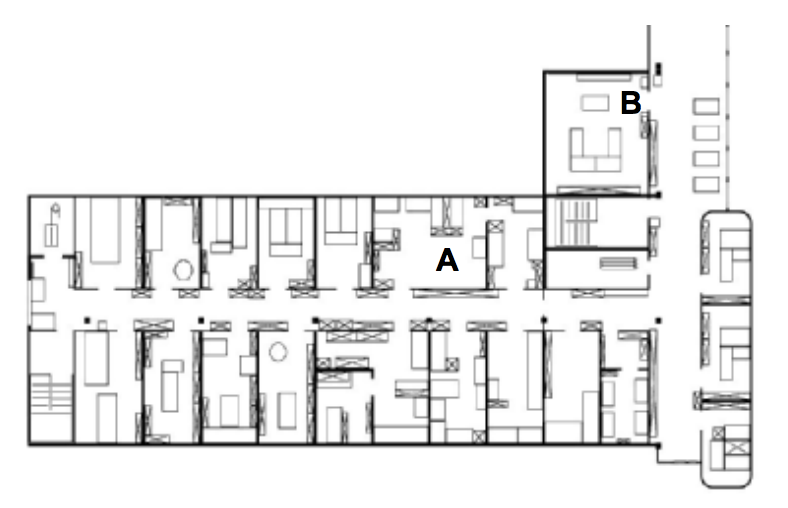
\includegraphics[width=0.6\textwidth]{img/Siegwart_5_6.png}
    \caption{Siegwart Figure 5.6. An environment with rooms A and B}
    \label{fig:siegwart_5_6}
\end{figure}

Behavioral approach attempts to design a set of behaviors that result in desired robot motion and trajectory. This method avoids mapping the robot's environment for localization. For example, consider Fig.~\ref{fig:siegwart_5_6}, where a robot wants to navigate from room A to room B. Using behavioral approach, a robot may find its way to room B by following the left wall, incorporating other procedures such as collision avoidance and identification of room B. However, compared to map-based approach, this method of navigation has difficulty scaling to different problems or environments. Depending on situations, techniques like following the left wall can also be suboptimal.

\subsection{Map-based Approach}

Map-based localization uses information about the robot's surrounding to identify its position \textit{with respect to} the environment. To gain knowledge of its environment, the robot must actively gather and process sensor data of the surrounding. The most popular sensor is LIDAR, which can provide $360^\circ$ coverage of the robot's surrounding. This approach can scale to any kind of environment, because a robot can use same techniques and sensors to map its surrounding.

\begin{figure}[h!]
	\centering
    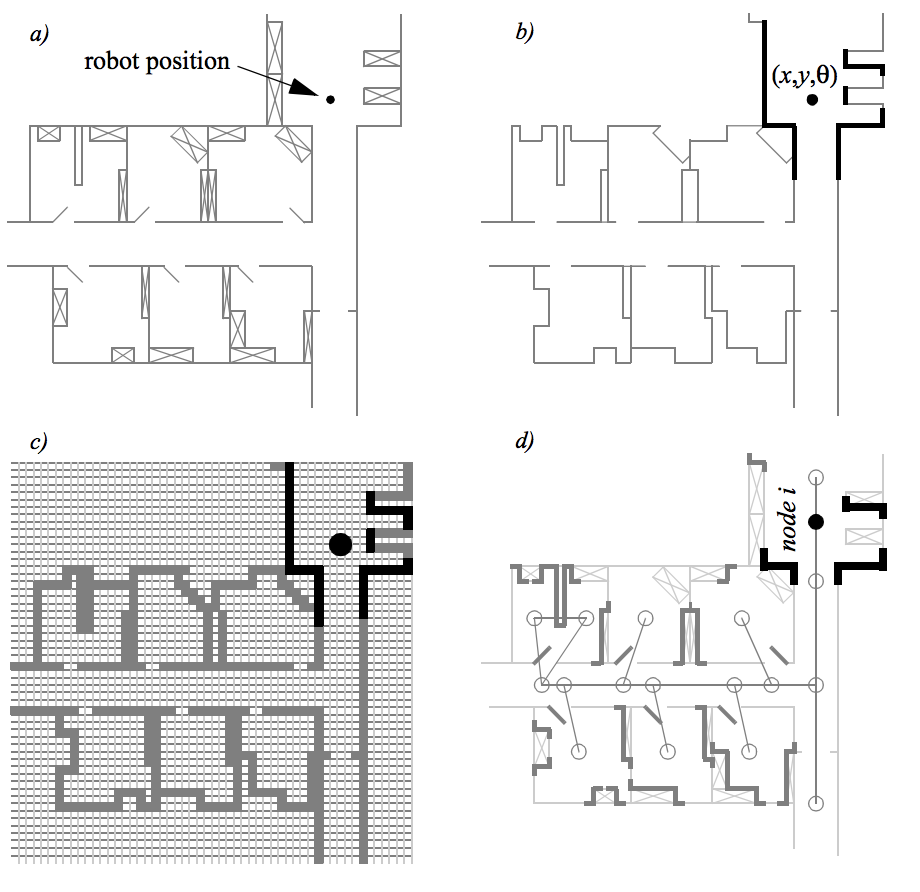
\includegraphics[width=0.8\textwidth]{img/Siegwart_maps.png}
    \caption{Siegwart Figure 5.10. (a) Real map. (b) Map where continuous lines represent walls. (c) Same map discretized into 3000 grid cells. (d) Topological map with nodes and edges.}
    \label{fig:siegwart_maps}
\end{figure}

\subsection{Belief representation}
Due to sensor noise, a robot cannot localize itself with absolute certainty. To compensate for the error, we can represent the estimate of robot's location as a probability distribution across the environment. There are different ways of representation. For example, the belief of robot's position can be \emph{continuous}, which can be expressed by continuous variables $(x, y, \theta)$ Fig.~\ref{fig:siegwart_maps}(b). \\

On the other hand, the belief can be \emph{discrete}. For instance, the map of the environment may be discretized into $N \times N$ cells as in Fig.~\ref{fig:siegwart_maps}(c), and the belief can assign probabilities of being in different cells. The other possible discrete representation is a topological map in Fig.~\ref{fig:siegwart_maps}(d), which maps the environment using nodes and edges. We can then assign probabilities of robot being in certain nodes. \\

\begin{figure}[h!]
	\centering
    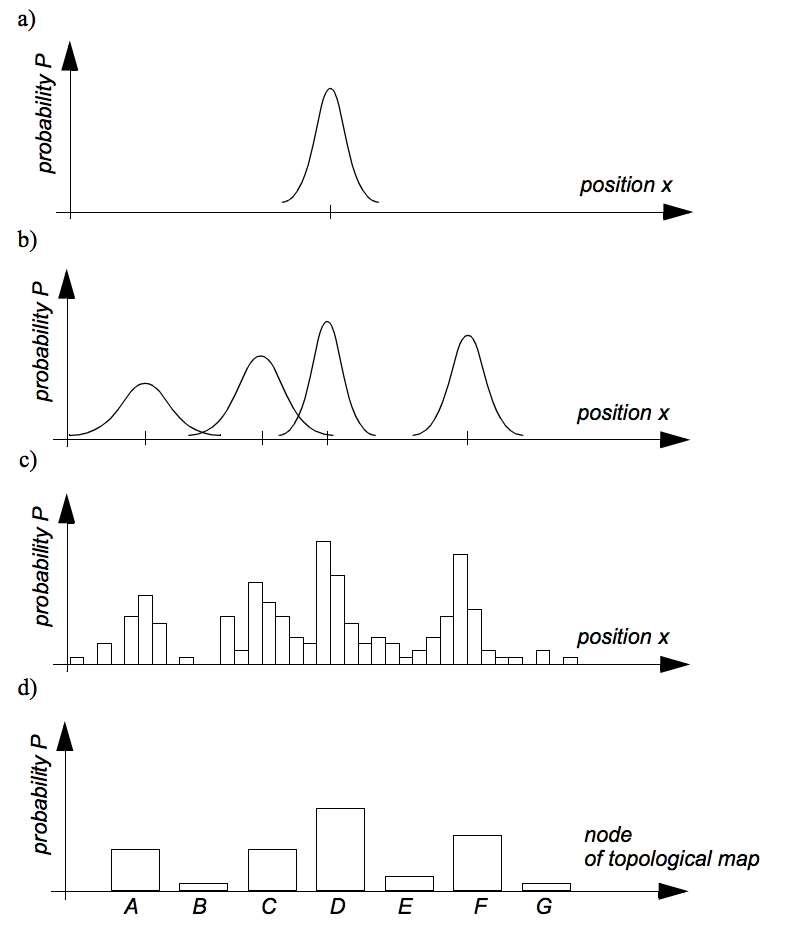
\includegraphics[width=0.8\textwidth]{img/Siegwart_beliefs.png}
    \caption{Siegwart Figure 5.9. (a) Continuous single-hypothesis belief. (b) Continuous multiple-hypothesis belief. (c) Discrete probabilities for grid-based map. (d) Discrete probabilities for topological map.}
    \label{fig:siegwart_beliefs}
\end{figure}

The belief representation can also be classified as either \emph{single-hypothesis belief} or \emph{multiple-hypothesis belief}. \emph{Single-hypothesis belief}, as in Fig.~\ref{fig:siegwart_beliefs}(a), is useful when describing a unique estimate of a robot's position. On the other hand, \emph{multiple-hypothesis belief} in Fig.~\ref{fig:siegwart_beliefs}(b, c, d) can be used to describe multiple possible locations of a robot. \\

Continuous belief representation typically incorporates single-hypothesis belief (ex. state vector [$x, y, \theta$]) that is compact and easy to compute. However, discrete belief representation typically incorporates multiple-hypothesis belief. Because discrete method assigns the probabilities of robot's presence across different cells or nodes in the map, we see that the accuracy of estimate is limited by the resolution of discretization. It may also involve heavy computation, because a robot must keep track of probabilities associated each cell \cite{Clark}.

\section{Probability Basics}

\subsection{Random Variable}

Quantities such as sensor measurements, states of a robot and its environment are modeled as random variables. A random variable is a variable whose possible values are outcomes of a random phenomenon. In the case of sensor measurements, the source of randomness could be sensor noise. Random variables fall under one of two categories: discrete or continuous.

\subsubsection{Discrete Random Variable}

Discrete random variables can take on only a countable number of values. For example, if we flip a coin twice and the random variable $X$ represents the number of coin flips resulting in "heads", $X$ can only take on values of 0, 1 or 2 (and similarly for the case of "tails"). A discrete random variable is characterized by a probability mass function (PMF) $p(X=x)$ (or $p(x)$) where
\begin{center}
$\sum\limits_{x} p(x)=1$.
\end{center}

\subsubsection{Continuous Random Variable}

In contrast with a discrete random variable, a continuous random variable can take on an infinite number of values. A continuous random variable is characterized by a probability density function (PDF), $p(x)$, where the probability of a random variable being contained within the interval $[a,b]$ is
\begin{center}
$P(a \leq X \leq b) = \int_{a}^{b}p(x)dx$
\end{center}
where
\begin{center}
$\int_{-\infty}^{+\infty}p(x)dx=1$.
\end{center}

\subsection{Joint Distributions, Independence and Conditional Probability}

\subsubsection{Joint Distributions}

The joint distribution of two random variables $X$ and $Y$ is denoted as \begin{center}
$p(x,y):=p(X=x\ \textnormal{and}\ Y=y).$
\end{center}

\subsubsection{Independence}

If $X$ and $Y$ are random variables such that,
\begin{center}
$p(x,y)=p(x)p(y)$
\end{center}
then $X$ and $Y$ are said to be independent.

\subsubsection{Conditional Probability}

Conditional probability is the probability of an event happening given that another event has occurred. That is, suppose that we know that the event $Y = y$ occurs with probability $p(y) > 0$. The probability of the event $X=x$ occurring given that $Y=y$ has occurred, or alternatively stated as the conditional probability of $X$ given $Y$, is given by

\begin{center}
$p(x|y):=\frac{p(x,y)}{p(y)}.$
\end{center}

Thus if $X$ and $Y$ are independent, $p(x|y)=p(x)$. Also, note that the above definition of conditional probability is indeed a definition and not theoretically derived.

In order to better understand the concept of conditional probability, consider Fig. ~\ref{fig:cond_prob_example}\. In this figure, the sample space $\Omega$ contain the set of all possible outcomes for a random variable. Consider the case where there are two possible outcomes, $B1$ and $B2$ which may occur with an equal probability of $0.5$. These events correspond to the orange and blue regions of $\Omega$, respectively. An event $A$ that occurs with probability $0.5$ can also be defined, which corresponds to the centered shaded region in Fig. ~\ref{fig:cond_prob_example}.

Suppose that we wish to determine the probability of $A$ occurring and that a sample from $\Omega$ is observed to result in the event $B1$. Given that $B1$ has occurred, we restrict our attention to the region $B1$. In this restricted region, the area corresponding to $A$ occurring is the intersection of $A$ and $B1$. Since region $A$ overlaps with half of the region $B1$, we have the result that $p(A|B1) = 0.5.$ A slightly different but equivalent interpretation of this figure, as given during lecture, is that we rescale the probability of event $A$ occurring by the probability of the event that has happened. Mathematically, this is expressed as

\begin{center}
$p(A|B1)=\frac{p(A \cap B1)}{p(B1)}=\frac{0.25}{0.5}=0.5.$
\end{center}

\begin{figure}[h!]
	\centering
    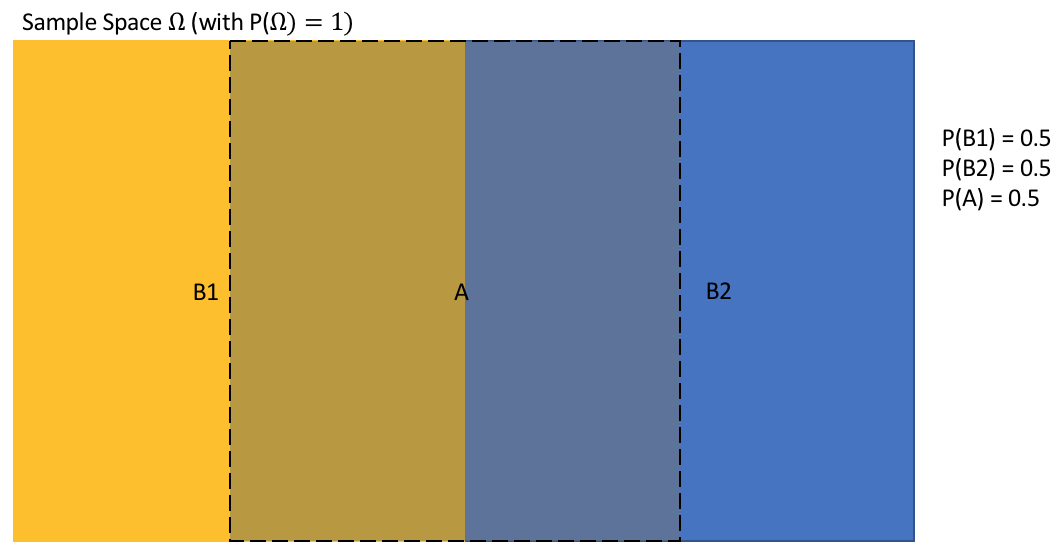
\includegraphics[width=0.6\textwidth]{img/Cond_Prob_Example.png}
    \caption{Sample space representation. Note that region A is centered an overlaps $B1$ and $B2$ equally.}
    \label{fig:cond_prob_example}
\end{figure}

Finally, note that if $X$ and $Y$ are independent $p(x|y):=p(x)$.
\subsubsection{Conditional Independence}
If $X$, $Y$ and $Z$ are random variables such that,
\begin{center}
$p(x,y \mid z)=p(x \mid z)p(y \mid z)$
\end{center}
then $X$ and $Y$ are said to be conditionally independent given $Z$. \newline
However:
\begin{center}
$p(x,y \mid z)=p(x \mid z)p(y \mid z) \not \Rightarrow p(x,y)=p(x)p(y)$
\end{center}
Nor:
\begin{center}
$p(x,y)=p(x)p(y) \not \Rightarrow p(x,y \mid z)=p(x \mid z)p(y \mid z)$
\end{center}
\subsection{Theorem of Total Probability}

Once again consider Fig. ~\ref{fig:cond_prob_example}. If we wished to find the probability of $A$ without any assumptions regarding conditioning, we can do so by calculating

\begin{center}
$p(A)=p(A \cap B1) + p(A \cap B2).$
\end{center}

This idea can be generalized for discrete random variables into what is known as the theorem (or law) of total probability as

\begin{center}
$p(x)=\sum\limits_{y}p(x,y)=\sum\limits_{y}p(x|y)p(y)$
\end{center}

where the definition of conditional probability was used to obtain the last expression. For continuous random variables, the summations simply turn into integrals:

\begin{center}
$p(x)=\int p(x,y)dy=\int p(x|y)p(y)dy$
\end{center}

\subsection{Bayes' Rule}

To facilitate the explanation of Bayes' Rule please note: a sample space is a set containing all the possible outcomes of an experiment and an event is a subset of elements in a sample space. Imagine that there is an event $A$ whose set of outcomes is contained in the sets of events $B_i$ where $i = 0, 1, ..., n$ of a sample space. For example in Fig. ~\ref{fig:cond_prob_example}\ event A's set is contained in the sets of events $B_1$ and $B_2$. Then,

\begin{center}
$p(B_i|A)=\frac{p(B_i \cap A)}{p(A)}$.
\end{center}

Using the formula for conditional probability $p(B_i \cap A)$ and $p(A)$ can be expressed as:

\begin{center}
$p(B_i \cap A)= p(A|B_i)p(B_i) $.

$p(A)= \sum\limits_{i = 0}^{n} p(B_i \cap A) = \sum\limits_{i = 0}^{n} p(A|B_i)p(B_i)$.
\end{center}

Combining these two expressions to derive Bayes' Rule for discrete sample spaces:

\begin{center}
$p(B_i|A)= \frac{p(A|B_i)p(B_i)}{\sum\limits_{i = 0}^{n} p(A|B_i)p(B_i)}$.
\end{center}

For a continuous sample space Bayes' Rule is:

\begin{center}
$p(B|A)= \frac{p(A|B)p(B)}{\int p(A|B = b')p(B = b')db'}$.
\end{center}

Note that $p(A)$ is independent of which event $Bi$ is selected. So the denominator of Bayes' formula can be considered a constant for all events $Bi$ with event $A$. Furthermore, by knowing the probabilities $p(A|Bi)$ and $p(Bi)$, we can determine $p(Bi|A)$. As an example, a brewery buys equal amounts of hops from two farmers, $B1$ and $B2$. The brewery has a strict policy of using only one type of hops in each batch of beer it brews. Furthermore, the brewery uses half of all its hops from both sources to produce Pilsner beer. Bayes' Rule can be applied to determine, given that a batch of Pilsner is produced, what is the probability that the batch was brewed using hops from farmer $B1$. Note this example uses the sample space described in Fig. ~\ref{fig:cond_prob_example}\

\begin{center}
$p(B_1|A)= \frac{p(A|B_1)p(B_1)}{\sum\limits_{i = 0}^{1} p(A|B_i)p(B_i)} = \frac{p(A|B_1)p(B_1)}{p(A|B_1)p(B_1) + p(A|B_2)p(B_2)} = \frac{0.5*0.5}{(0.5*0.5 + 0.5*0.5)} = \frac{0.25}{0.5} = 0.5$.
\end{center}

Bayes' Rule can be extended with the use of additional random variables. In the three variable case, given $X=x$, $Y=y$ Bayes' Rule can be conditioned on an additional variable $Z=z$ as follows:

\begin{center}
$p(x|y, z)= \frac{p(y|x,z)p(x|z)}{p(y|z)}$.
\end{center}

This is the probability that event $Z=z$, and event $X=x|Y=y$ occur, which describes $Z=z$ influence on joint event $X=x|Y=y$.

\subsection{Expectation and Covariance}

The expectation value of a random variable $E(X)$ is the average result of an experiment over an infinite number of trials. It is also known as the first moment of the distribution. For the discrete case:

\begin{center}
$E(X)= \sum\limits_{i = 0}^{n} x_ip(X=x_i)$.
\end{center}

For the continuous case:

\begin{center}
$E(X)= \int\limits_{-\infty}^{\infty}  x'p(X=x')dx'$.
\end{center}

The expectation value of a constant is a constant and its calculation is a linear operation.

\begin{center}
$E(aX + b)= aE(X) + b$.
\end{center}

In the case of a vector of random variables. The expectation of the vector is the vector of each variables expectation value.

Covariance is a calculation used to measure the relationship between random variables. For two random variable vectors $X=x, Y=y$, the covariance is:

\begin{center}
$cov(X,Y)=E[(X-E(X))(Y-E(Y))] = E(XY^T) - E(X)E(Y^T)$
\end{center}

If the covariance is positive this implies that X tends to increase at the same time as Y. If the covariance is negative then this implies that X tends to decrease as Y increases.If changes in X and Y have a random relationship, then the covariance will be close to zero. If two variables have a covariance of zero they are called uncorrelated. If two variables are independent they will be uncorrelated. However, two variables which are uncorrelated are not always independent.

\bibliographystyle{ieee}
\bibliography{egbib}

\subsubsection*{Contributors}
Winter 2019: [Your Names Here]
\\
Winter 2018: Junjie Ke, Ryan Wong, Amine Elhafsi, Samuel Sowell, Peter Zachares
\end{document}
